% Choose one to switch betweeen slides and handout
\documentclass[]{beamer}
%\documentclass[handout]{beamer}

% Video Meta Data
\title{Bitcoin, Blockchain and Cryptoassets}
\subtitle{Monetary Control Structures}
\author{Prof. Dr. Fabian Schär}
\institute{University of Basel}

% Config File
% Packages
\usepackage[utf8]{inputenc}
\usepackage{hyperref}
\usepackage{gitinfo2}
\usepackage{tikz}
\usepackage{amsmath}
\usepackage{bibentry}
\usepackage{xcolor}
\usepackage{colortbl} % Add colour to LaTeX tables
\usepackage{caption}
\usepackage[export]{adjustbox}
\usepackage{pgfplots} \pgfplotsset{compat = 1.17}

% Color Options
\definecolor{highlight}{rgb}{0.65,0.84,0.82}
\definecolor{focus}{rgb}{0.72, 0, 0}

% Beamer Template Options
\beamertemplatenavigationsymbolsempty
\setbeamertemplate{footline}[frame number]
\setbeamercolor{structure}{fg=black}
\setbeamercolor{footline}{fg=black}
\setbeamercolor{title}{fg=black}
\setbeamercolor{frametitle}{fg=black}
\setbeamercolor{item}{fg=black}
\setbeamercolor{}{fg=black}
\setbeamercolor{bibliography item}{fg=black}
\setbeamercolor*{bibliography entry title}{fg=black}
\setbeamertemplate{items}[square]
\setbeamertemplate{enumerate items}[default]
\captionsetup[figure]{labelfont={color=black},font={color=black}}
\captionsetup[table]{labelfont={color=black},font={color=black}}

\setbeamertemplate{bibliography item}{\insertbiblabel}

% Link Icon Command
\newcommand{\link}{%
    \tikz[x=1.2ex, y=1.2ex, baseline=-0.05ex]{%
        \begin{scope}[x=1ex, y=1ex]
            \clip (-0.1,-0.1)
                --++ (-0, 1.2)
                --++ (0.6, 0)
                --++ (0, -0.6)
                --++ (0.6, 0)
                --++ (0, -1);
            \path[draw,
                line width = 0.5,
                rounded corners=0.5]
                (0,0) rectangle (1,1);
        \end{scope}
        \path[draw, line width = 0.5] (0.5, 0.5)
            -- (1, 1);
        \path[draw, line width = 0.5] (0.6, 1)
            -- (1, 1) -- (1, 0.6);
        }
    }

% Read Git Data from Github Actions Workflow
% Defaults to gitinfo2 for local builds
\IfFileExists{gitInfo.txt}
	{\input{gitInfo.txt}}
	{
		\newcommand{\gitRelease}{(Local Release)}
		\newcommand{\gitSHA}{\gitHash}
		\newcommand{\gitDate}{\gitAuthorIsoDate}
	}

% Custom Titlepage
\defbeamertemplate*{title page}{customized}[1][]
{
  \vspace{-0cm}\hfill
\includegraphics[width=2.5cm]{../config/logo_cif}
  
\includegraphics[width=1.9cm]{../config/seal_wwz}
  \\ \vspace{2em}
  \usebeamerfont{title}\textbf{\inserttitle}\par
  \usebeamerfont{title}\usebeamercolor[fg]{title}\insertsubtitle\par  \vspace{1.5em}
  \small\usebeamerfont{author}\insertauthor\par
  \usebeamerfont{author}\insertinstitute\par \vspace{2em}
  \usebeamercolor[fg]{titlegraphic}\inserttitlegraphic
    \tiny \noindent \texttt{Release Ver.: \gitRelease}\\ 
    \texttt{Version Hash: \gitSHA}\\
    \texttt{Version Date: \gitDate}\\ \vspace{1em}
  \link \href{https://github.com/cifunibas/Bitcoin-Blockchain-Cryptoassets/blob/main/slides/intro.pdf}
  {Get most recent version}\\
  \link \href{https://github.com/cifunibas/Bitcoin-Blockchain-Cryptoassets/blob/main/slides/intro.pdf}
  {Watch video lecture}\\ \vspace{1em}
  License: \texttt{Creative Commons Attribution-NonCommercial-ShareAlike 4.0 International}\\\vspace{2em}
  
\includegraphics[width = 1.2cm]{../config/license}
}

% tikzlibraries
\usetikzlibrary{decorations.pathreplacing}
\usetikzlibrary{decorations.markings}
\usetikzlibrary{positioning}

%caption font
\captionsetup{font=footnotesize}


%%%%%%%%%%%%%%%%%%%%%%%%%%%%%%%%%%%%%%%%%%%%%%
%%%%%%%%%%%%%%%%%%%%%%%%%%%%%%%%%%%%%%%%%%%%%%
\begin{document}

\thispagestyle{empty}
\begin{frame}[noframenumbering]
	\titlepage
\end{frame}

%%%
\begin{frame}{Monetary Control Structures}
	Monetary control structures can be described along three dimensions:
	\vspace{1.5em}
	\begin{figure}
		\begin{tikzpicture}[align = center]
	
	% define coordinates
	\coordinate (1) at (-3, 0);
	\coordinate (2) at (0, 0);
	\coordinate (3) at (3, 0);
	
	% creation
	\node[left] at (1) {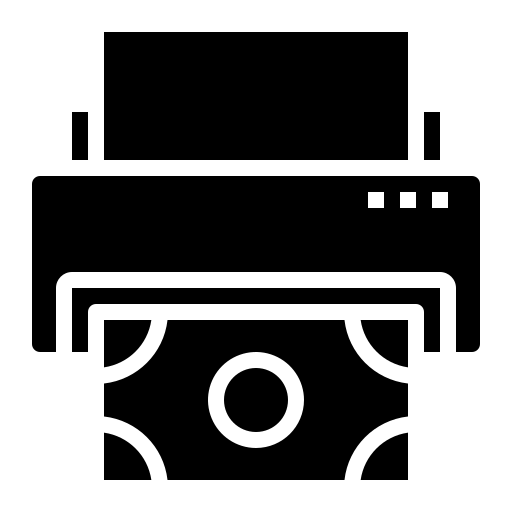
\includegraphics[height = 0.1\textheight]{../assets/images/creation}};
	\node[right] at (1) {
\includegraphics[height = 0.1\textheight]{../assets/images/agents/miner_right}};
	\node[below = 18pt] at (1) {Creation};

	% representation
	\uncover<2->{
		\node[left] at (2) {
\includegraphics[height = 0.1\textheight]{../assets/images/currency}};
		\node[right] at (2) {
\includegraphics[height = 0.1\textheight]{../assets/images/virtual}};
		\node[below = 18pt] at (2) {Representation};
	}
	
	% transaction processing
	\uncover<3->{
		\node[left] at (3) {
\includegraphics[height = 0.1\textheight]{../assets/images/agents/intermediary}};
		\node[right] at (3) {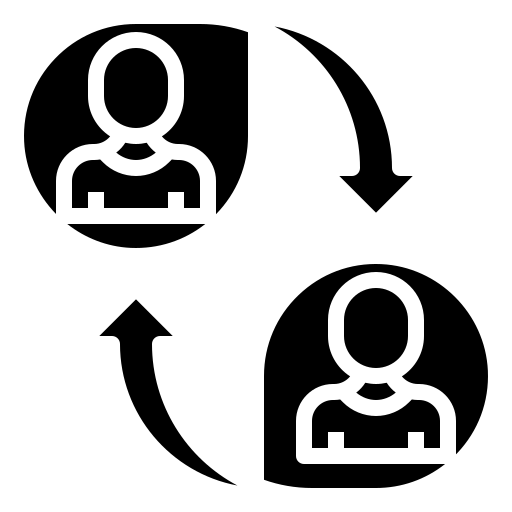
\includegraphics[height = 0.1\textheight]{../assets/images/peer-to-peer}};
		\node[below = 12pt] at (3) {Transaction\\ processing};
	}
	
\end{tikzpicture}
	\end{figure}
\end{frame}
%%%

%%%
\begin{frame}{Matrix of the Control Structures}
	\begin{figure}
		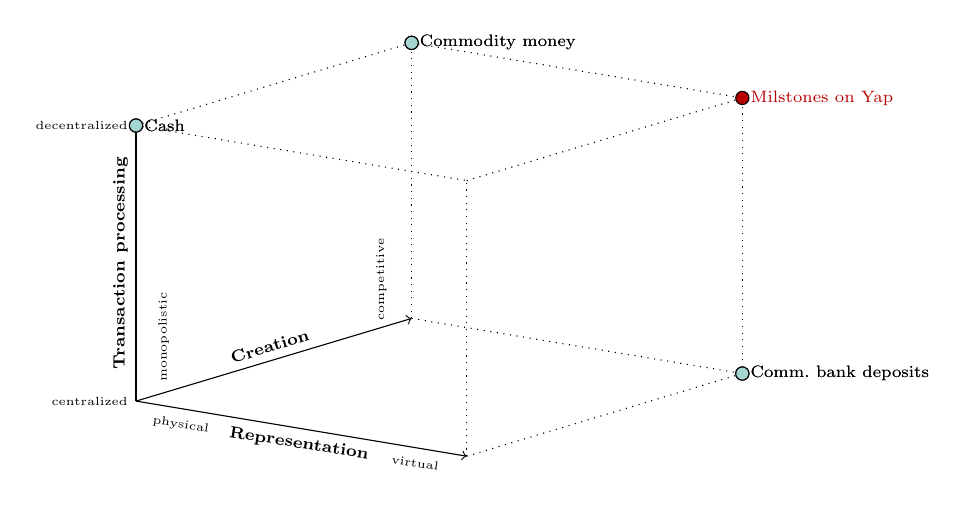
\begin{tikzpicture}[scale = 0.7, every node/.style={scale=0.85}]

	\draw[color=black, ->] (0,0) -- (6,-1);
    \draw[color=black] plot (3,-0.5) node[color=black,below, rotate = -9] {\scriptsize{\textbf{Representation}}};
    
     \draw[color=black, ->] (0,0) -- (0,5);
     \draw[color=black] plot (0,2.5) node[color=black,above, rotate = 90] {\scriptsize{\textbf{Transaction processing}}};
     
     \draw[color=black, ->] (0,0) -- (5,1.5);
     \draw[color=black] plot (2.5,0.75) node[color=black, above, rotate = 17] {\scriptsize{\textbf{Creation}}};
     
     \draw[color=black, dotted] (0,5) -- (6, 4);
     \draw[color=black, dotted] (6,-1) -- (6, 4);
     \draw[color=black, dotted] (5,1.5) -- (11, 0.5);
     \draw[color=black, dotted] (0,5) -- (5, 6.5);
     \draw[color=black, dotted] (5,1.5) -- (5, 6.5);
     \draw[color=black, dotted] (5,6.5) -- (11, 5.5);
     \draw[color=black, dotted] (11,0.5) -- (11, 5.5);
     \draw[color=black, dotted] (6,-1) -- (11, 0.5);
     \draw[color=black, dotted] (6,4) -- (11, 5.5);
     
     \uncover<2->{\alt<2>{\draw[fill=focus] (0,5) circle (0.12cm) node[right,color=black] {\scriptsize{Cash}};}{\draw[fill=highlight] (0,5) circle (0.12cm) node[right,color=black] {\scriptsize{Cash}};}}
     
     \uncover<3->{\alt<3>{\draw[fill=focus] (5,6.5) circle (0.12cm) node[right,color=black] {\scriptsize{Commodity money}};}{\draw[fill=highlight] (5,6.5) circle (0.12cm) node[right,color=black] {\scriptsize{Commodity money}};}}
     
     \uncover<4->{\alt<4>{\draw[fill=focus] (11,0.5) circle (0.12cm) node[right,color=black] {\scriptsize{Comm.\ bank deposits}};}{\draw[fill=highlight] (11,0.5) circle (0.12cm) node[right,color=black] {\scriptsize{Comm.\ bank deposits}};}}
     
     \uncover<5->{\draw[fill=focus] (11,5.5) circle (0.12cm) node[right,color=focus] {\scriptsize{Milstones on Yap}};}

     \draw[color=black] plot (0,0)                  node[left, rotate = 0] {\tiny{centralized}};
     \draw[color=black] plot (0,5)                  node[left, rotate = 0] {\tiny{decentralized}};
     
     \draw[color=black] plot (0.5,0.2)                  node[right, rotate = 90] {\tiny{monopolistic}};
     \draw[color=black] plot (4.45,3.1)                  node[left, rotate = 90] {\tiny{competitive}};
          
     \draw[color=black] plot (0.85,-0.19)                  node[below, rotate = -9] {\tiny{physical}};
     \draw[color=black] plot (5.1,-0.9)                  node[below, rotate = -9] {\tiny{virtual}};
     
\end{tikzpicture}
	\end{figure}
\end{frame}
%%%

%%%
\begin{frame}{Competitive Creation}
	\begin{columns}
		\begin{column}{0.5\textwidth}
			\begin{figure}
				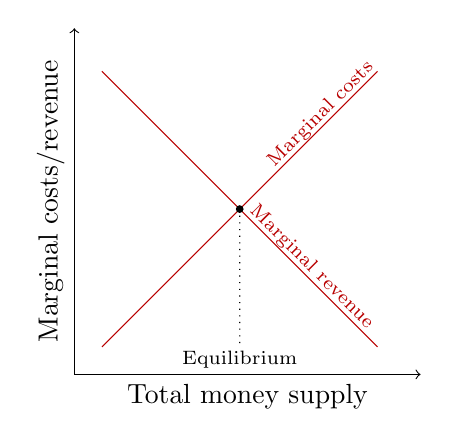
\begin{tikzpicture}[scale = 0.7]

	% define coordinates
			\coordinate (0) at (0,0);
			\coordinate (1x) at (6,0);
			\coordinate (1y) at (0,6);
			\coordinate (mid) at (3,3);
		
		% draw axes
			\draw[->] (0) -- ([xshift = 8pt] 1x) node[midway, below] {Total money supply};
			\draw[->] (0) -- ([yshift = 8pt] 1y) node[midway, above, rotate = 90] {Marginal costs/revenue};
		
		% MC
			\draw[focus] (0.5, 0.5) -- (5.5, 5.5) node[rotate = 45, above = 5pt, left]{\scriptsize{Marginal costs}};
			
		% MR
			\draw[focus] (0.5, 5.5) -- (5.5, 0.5) node[rotate = -45, above = 5pt, left]{\scriptsize{Marginal revenue}};
			
		% Equilibrium
			\fill[fill, circle] (mid) circle[radius = 2pt];
			\draw[dotted] (mid) -- (3, 0.5) node[below = -2pt]{\scriptsize{Equilibrium}};
			
\end{tikzpicture}
				\caption*{(a) Increasing marginal costs}
			\end{figure}
		\end{column}
		\begin{column}{0.5\textwidth}
			\begin{figure}
				\uncover<2->{
					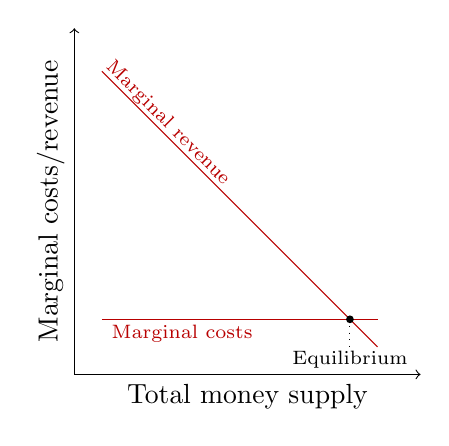
\begin{tikzpicture}[scale = 0.7]

	% define coordinates
			\coordinate (0) at (0,0);
			\coordinate (1x) at (6,0);
			\coordinate (1y) at (0,6);
			\coordinate (mid) at (3,3);
		
		% draw axes
			\draw[->] (0) -- ([xshift = 8pt] 1x) node[midway, below] {Total money supply};
			\draw[->] (0) -- ([yshift = 8pt] 1y) node[midway, above, rotate = 90] {Marginal costs/revenue};
		
		% MC
			\draw[focus] (0.5, 1) node[below = 5pt, right]{\scriptsize{Marginal costs}} -- (5.5, 1) ;
			
		% MR
			\draw[focus] (0.5, 5.5) node[rotate = -45, above = 5pt, right]{\scriptsize{Marginal revenue}} -- (5.5, 0.5);
			
		% Equilibrium
			\fill[fill, circle] (5,1) circle[radius = 2pt];
			\draw[dotted] (5, 1) -- (5, 0.5) node[below = -2pt]{\scriptsize{Equilibrium}};
			
\end{tikzpicture}
					\caption*{(b) Constant marginal costs}
				}
			\end{figure}
		\end{column}
	\end{columns}
\end{frame}
%%%

%%%
\begin{frame}{Monopolistic Creation}
	\begin{figure}
		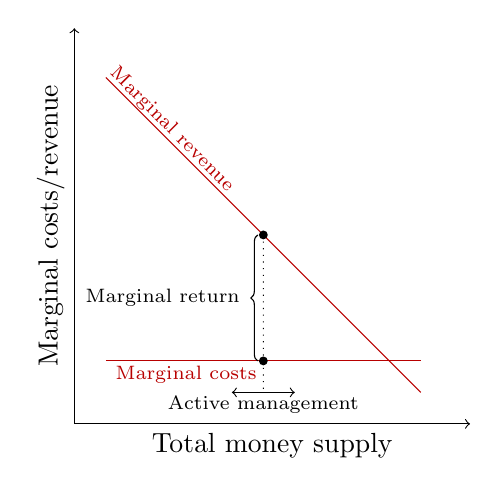
\begin{tikzpicture}[scale = 0.8]

	% define coordinates
			\coordinate (0) at (0,0);
			\coordinate (1x) at (6,0);
			\coordinate (1y) at (0,6);
			\coordinate (mid) at (3,3);
		
		% draw axes
			\draw[->] (0) -- ([xshift = 8pt] 1x) node[midway, below] {Total money supply};
			\draw[->] (0) -- ([yshift = 8pt] 1y) node[midway, above, rotate = 90] {Marginal costs/revenue};
		
		% MC
			\draw[focus] (0.5, 1) node[below = 5pt, right ]{\scriptsize{Marginal costs}} -- (5.5, 1) ;
			
		% MR
			\draw[focus] (0.5, 5.5) node[rotate = -45, above = 5pt, right]{\scriptsize{Marginal revenue}} -- (5.5, 0.5);
			
		% Active management
			\fill[fill, circle] (3,1) circle[radius = 2pt];
			\fill[fill, circle] (mid) circle[radius = 2pt];
			\draw[dotted] (mid) -- (3,0.5) node[below = -2pt]{\scriptsize{Active management}};
			\draw[decoration={brace, mirror, raise = 2pt}, decorate]
  (mid) -- (3,1) node[midway, left = 5pt] {\scriptsize{Marginal return}};
  			\draw[<->] (2.5,0.5) -- (3.5,0.5);
			
\end{tikzpicture}
		\caption*{Monopolistic money creation with constant marginal costs}
	\end{figure}
\end{frame}
%%%

%%%
\begin{frame}{Physical Representation}
	Physical monetary units are tied to an object.
	\vspace{1em}
	\begin{figure}
		\centering
		
\includegraphics[height = 0.15\textheight]{../assets/images/currency}
	\end{figure}
	\vspace{1em}
	\begin{columns}
		\begin{column}{0.5\textwidth}
			\uncover<2->{
				\textbf{Pros:}
				\begin{itemize}
					\item Simple
					\item Clear ownership rights
					\item Anonymity
					\item No systemic dependency
				\end{itemize}
			}
		\end{column}
		\begin{column}{0.5\textwidth}
			\uncover<3->{
				\textbf{Cons:}
				\begin{itemize}
					\item Location bound
					\item Safekeeping and transport
					\item Counterfeiting
					\item Divisibility
				\end{itemize}
			}
		\end{column}	
	\end{columns}
\end{frame}
%%%

%%%
\begin{frame}{Virtual Representation}
	Virtual monetary units allow the transfer of value without any change in the physical control of a particular object.
	\vspace{1em}
	\begin{figure}
		\centering
		
\includegraphics[height = 0.15\textheight]{../assets/images/virtual}
	\end{figure}
	\vspace{1em}
	\begin{columns}
		\begin{column}{0.5\textwidth}
			\uncover<2->{
				\textbf{Pros:}
				\begin{itemize}
					\item No physical handover
				\end{itemize}
			}
		\end{column}
		\begin{column}{0.5\textwidth}
			\uncover<3->{
				\textbf{Cons:}
				\begin{itemize}
					\item Contestable
				\end{itemize}
			}
		\end{column}	
	\end{columns}
\end{frame}
%%%

%%%
\begin{frame}{Transaction Processing}
	\begin{columns}[T]
		\begin{column}{0.5\textwidth}
			\center
			\textbf{Decentralized}
			\begin{figure}
				\begin{tikzpicture}[scale = 1.5]
	
	% define coordinates
	\coordinate (0) at (0,0);
	\coordinate (1) at (1,0);
	
	\node at (0){
\includegraphics[height = 0.15\textheight]{../assets/images/agents/handing_money_right}};
	\node at (1){
\includegraphics[height = 0.15\textheight]{../assets/images/agents/reaching_left}};
	
\end{tikzpicture}
			\end{figure}
		\end{column}
		\begin{column}{0.5\textwidth}
			\uncover<2->{
				\center
				\textbf{Centralized}
				\begin{figure}
					\begin{tikzpicture}
	
	% define coordinates
	\coordinate (0) at (0,0);
	\coordinate (1) at (1,0);
	\coordinate (2) at (2,0);
	
	\node at (0){
\includegraphics[height = 0.1\textheight]{../assets/images/agents/handing_money_right}};
	\node at (1){\alt<5>{
\includegraphics[height = 0.1\textheight]{../assets/images/agents/intermediary_devil}}{
\includegraphics[height = 0.1\textheight]{../assets/images/agents/intermediary}}};	
	\node at (2){
\includegraphics[height = 0.1\textheight]{../assets/images/agents/reaching_left}};
	
\end{tikzpicture}
				\end{figure}
			}
		\end{column}
	\end{columns}
	\vspace{1.5em}
	\uncover<3->{
	\vspace{1.5em}
	For virtual monetary units:
	\begin{center}
			\begin{tabular}{lccc}
				\hline \hline
					& Decentralized & Centralized \\
				Transaction capacity  & \uncover<6->{\checkmark} & \uncover<4->{\checkmark} \\
				Transaction legitimacy & \uncover<6->{\checkmark} & \uncover<4->{\checkmark} \\
				Transaction consensus & \uncover<6->{\textcolor{focus}?} & \uncover<4->{\checkmark} \\ \hline \hline
			\end{tabular}
		\end{center}
	}
\end{frame}
%%%

%%%
\begin{frame}{Desirable Control Structures}
	\begin{figure}
		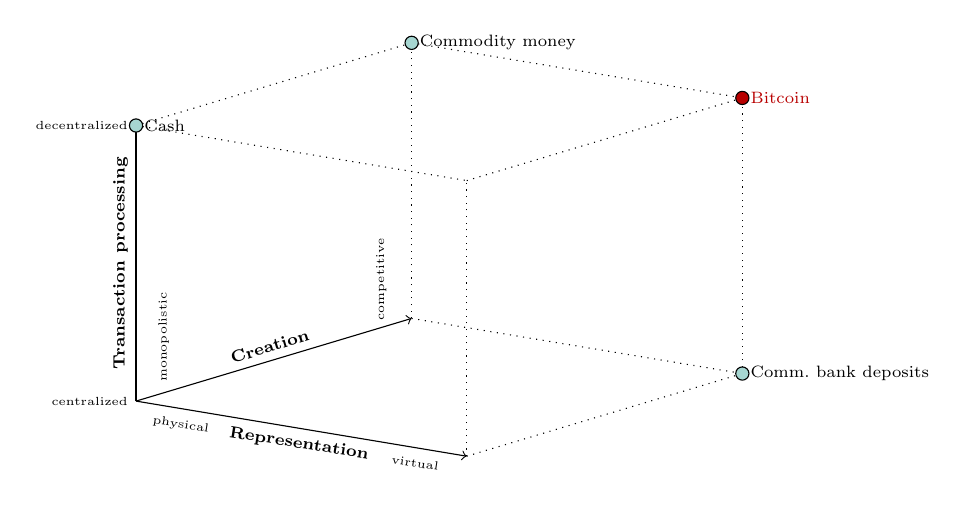
\begin{tikzpicture}[scale = 0.7, every node/.style={scale=0.85}]

	\draw[color=black, ->] (0,0) -- (6,-1);
    \draw[color=black] plot (3,-0.5) node[color=black,below, rotate = -9] {\scriptsize{\textbf{Representation}}};
    
     \draw[color=black, ->] (0,0) -- (0,5);
     \draw[color=black] plot (0,2.5) node[color=black,above, rotate = 90] {\scriptsize{\textbf{Transaction processing}}};
     
     \draw[color=black, ->] (0,0) -- (5,1.5);
     \draw[color=black] plot (2.5,0.75) node[color=black, above, rotate = 17] {\scriptsize{\textbf{Creation}}};
     
     \draw[color=black, dotted] (0,5) -- (6, 4);
     \draw[color=black, dotted] (6,-1) -- (6, 4);
     \draw[color=black, dotted] (5,1.5) -- (11, 0.5);
     \draw[color=black, dotted] (0,5) -- (5, 6.5);
     \draw[color=black, dotted] (5,1.5) -- (5, 6.5);
     \draw[color=black, dotted] (5,6.5) -- (11, 5.5);
     \draw[color=black, dotted] (11,0.5) -- (11, 5.5);
     \draw[color=black, dotted] (6,-1) -- (11, 0.5);
     \draw[color=black, dotted] (6,4) -- (11, 5.5);
     
	 \draw[fill=highlight] (0,5) circle (0.12cm) node[right,color=black] {\scriptsize{Cash}};
     
     \draw[fill=highlight] (5,6.5) circle (0.12cm) node[right,color=black] {\scriptsize{Commodity money}};
     
     \draw[fill=highlight] (11,0.5) circle (0.12cm) node[right,color=black] {\scriptsize{Comm.\ bank deposits}};
     
     \uncover<2->{\draw[fill=focus] (11,5.5) circle (0.12cm) node[right,color=focus] {\scriptsize{Bitcoin}};}

     \draw[color=black] plot (0,0) node[left, rotate = 0] {\tiny{centralized}};
     \draw[color=black] plot (0,5) node[left, rotate = 0] {\tiny{decentralized}};
     
     \draw[color=black] plot (0.5,0.2) node[right, rotate = 90] {\tiny{monopolistic}};
     \draw[color=black] plot (4.45,3.1) node[left, rotate = 90] {\tiny{competitive}};
          
     \draw[color=black] plot (0.85,-0.19) node[below, rotate = -9] {\tiny{physical}};
     \draw[color=black] plot (5.1,-0.9) node[below, rotate = -9] {\tiny{virtual}};
     
\end{tikzpicture}
	\end{figure}
\end{frame}
%%%

\end{document}